\def\regenfigs{0}
\documentclass[anonymous,sigconf,9pt]{acmart}

\usepackage{microtype}
\if\regenfigs1
\usepackage{tikz,pgfplots}
\usetikzlibrary{arrows.meta}
\usepgfplotslibrary{groupplots}
\usepgfplotslibrary{external}
\usepgfplotslibrary{colorbrewer}
\pgfplotsset{cycle list/Set1}
\usepgfplotslibrary{fillbetween}
\pgfplotsset{compat=1.18}
\pgfplotsset{
    tick align=outside,
    tick pos=left,
    xmajorgrids,
    x grid style={white},
    ymajorgrids,
    y grid style={white},
    axis line style={white},
    axis background/.style={fill=white!89.803921568627459!black},
    legend style={draw=none, fill=none},
    legend cell align=left,
}
\pgfkeys{/pgf/number format/.cd, 1000 sep={\,}}

\pgfplotsset{
    log x ticks with fixed point/.style={
        xticklabel={
            \pgfkeys{/pgf/fpu=true}
            \pgfmathparse{2^\tick}%
            \pgfmathprintnumber[fixed relative, precision=4]{\pgfmathresult}
            \pgfkeys{/pgf/fpu=false}
        }
    },
    log10 x ticks with fixed point/.style={
        xticklabel={
            \pgfkeys{/pgf/fpu=true}
            \pgfmathparse{10^\tick}%
            \pgfmathprintnumber[fixed relative, precision=3]{\pgfmathresult}
            \pgfkeys{/pgf/fpu=false}
        }
    },
    log y ticks with fixed point/.style={
        yticklabel={
            \pgfkeys{/pgf/fpu=true}
            \pgfmathparse{2^\tick}%
            \pgfmathprintnumber[fixed relative, precision=4]{\pgfmathresult}
            \pgfkeys{/pgf/fpu=false}
        }
    }
}
\fi

\begin{document}

\definecolor{eos}{RGB}{35,139,69}
\definecolor{alps}{RGB}{35,139,69}
\definecolor{aurora}{RGB}{107,174,214}
\definecolor{frontier}{RGB}{239,59,44}
\definecolor{elcap}{RGB}{253,141,60}
\begin{figure*}[tbp]
\if\regenfigs1
\begin{tikzpicture}[overlay=false,>=latex]
    \begin{groupplot}[
            /tikz/overlay=false,
            /tikz/thick,
            group style={
                group size=3 by 1,
                vertical sep=0.2cm,
                horizontal sep=0.9cm,
                xlabels at=edge bottom,
                ylabels at=edge left,
                xticklabels at=edge bottom,
            },
            width=\linewidth/2,
            ylabel near ticks,
            xlabel={\# GPU nodes},
            xmode=log,
            ymode=log,
            log basis x=10,
            xmin=0.5, xmax=11000,
            %log10 x ticks with fixed point,
            clip=false,
            title style={yshift=-0.5cm, xshift=-2.1cm,anchor=west},
            %ylabel style={xshift=1.2cm},
            ylabel={timesteps/s},
            height=2.1in,
            width=2.5in,
        ]
            
            \nextgroupplot[
                ymin=0.2, ymax=5050,
                legend style={at={(0.7,0.3)},anchor=east},
                legend columns=1,
                title={a) LJ},
            ]
            %\addlegendimage{empty legend};
            %\addlegendentry{\hspace{-0.65cm}\# atoms};
            \addplot+[mark=*,frontier]  table[y index=2] {results_frontier/lj_1e7.txt};
            %\addlegendentry{Frontier};
            \addplot+[mark=triangle*,aurora]  table[y index=2] {results_aurora/lj_1e7.txt};
            %\addlegendentry{Aurora};
            
            \addplot+[mark=diamond*,elcap]  table[y expr={\thisrowno{1}*0.8192}] {results_elcap/lj_1e7.txt};
            \addplot+[mark=diamond*,elcap]  table[y expr={\thisrowno{1}*1.05}] {results_elcap/lj_1e9.txt};
            \addplot+[mark=diamond*,elcap]  table[y expr={\thisrowno{1}*1.342}] {results_elcap/lj_1e11.txt};
            
            \addplot+[mark=*,frontier]  table[y index=2] {results_frontier/lj_1e9.txt};
            \addplot+[mark=*,frontier]  table[y index=2] {results_frontier/lj_1e11.txt};
            
            % \addplot+[mark=square*,eos]  table[y expr={\thisrowno{2}*0.8192}] {results_eos/lj_8M.txt};
            % \addplot+[mark=square*,eos]  table[y expr={\thisrowno{2}*1.05}] {results_eos/lj_1B.txt};
            % \addplot+[mark=square*,eos]  table[y expr={\thisrowno{2}*1.342}] {results_eos/lj_128B.txt};
            
            \addplot+[mark=square*,alps]  table[y expr={\thisrowno{2}*0.8192}] {results_alps/lj-8M-4gpus.txt};
            \addplot+[mark=square*,alps]  table[y expr={\thisrowno{2}*1.05}] {results_alps/lj-1B-4gpus.txt};
            \addplot+[mark=square*,alps]  table[y expr={\thisrowno{2}*1.342}] {results_alps/lj-128B-4gpus.txt};

            \addplot+[mark=triangle*,aurora]  table[y index=2] {results_aurora/lj_1e9.txt};
            \addplot+[mark=triangle*,aurora]  table[y index=2] {results_aurora/lj_1e11.txt};
            
            \draw (axis cs:1,175) node[anchor=north] {\(10^7\)};
            \draw (axis cs:2,2) node[anchor=135] {\(10^9\) atoms};
            \draw (axis cs:128,1) node[anchor=north] {\(10^{11}\)};
            
            \nextgroupplot[
                ymin=0.4, ymax=205,
                legend style={at={(0.5,1.0)},anchor=south},
                legend columns=9,
                title={b) ReaxFF},
            ]
            %\addplot+[mark=square*,eos]  table[y expr={\thisrowno{2}*0.9339}] {results_eos/hns_1M.txt};
            %\addlegendentry{Eos (4\(\times\)H100)};
            %\addplot+[mark=*,frontier]  table[y index=2] {results_frontier/hns_1e6.txt};
            \addplot+[mark=square*,alps]  table[y expr={\thisrowno{2}*0.9339}] {results_alps/reaxff-1M-4gpus.txt};
            \addlegendentry{Alps (4\(\times\)GH200)};
            \addlegendentry{Frontier (4\(\times\)MI250X)};
            \addplot+[mark=diamond*,elcap]  table[y expr={\thisrowno{1}*0.9339}] {results_elcap/hns_1e6.txt};
            \addlegendentry{El Capitan (4\(\times\)MI300A)};
            \addplot+[mark=triangle*,aurora]  table[y index=2] {results_aurora/hns_1e6.txt};
            \addlegendentry{Aurora (6\(\times\)PVC)};
            
            \addplot+[mark=*,frontier]  table[y index=2] {results_frontier/hns_1e8.txt};
            \addplot+[mark=*,frontier]  table[y index=2] {results_frontier/hns_1e10.txt};
            
            %\addplot+[mark=square*,eos]  table[y expr={\thisrowno{2}*1.195}] {results_eos/hns_128M.txt};
            \addplot+[mark=square*,alps]  table[y expr={\thisrowno{2}*1.195}] {results_alps/reaxff-128M-4gpus.txt};
            \addplot+[mark=square*,alps]  table[y expr={\thisrowno{2}*1.53}] {results_alps/reaxff-16B-4gpus.txt};

            
            \addplot+[mark=diamond*,elcap]  table[y expr={\thisrowno{1}*1.195}] {results_elcap/hns_1e8.txt};
            \addplot+[mark=diamond*,elcap]  table[y expr={\thisrowno{1}*1.53}] {results_elcap/hns_1e10.txt};
            
            \addplot+[mark=triangle*,aurora]  table[y index=2] {results_aurora/hns_1e8.txt};
            \addplot+[mark=triangle*,aurora]  table[y index=2] {results_aurora/hns_1e10.txt};
            
            \draw (axis cs:1,18) node[anchor=north] {\(10^6\)};
            \draw (axis cs:4,0.96) node[anchor=north] {\(10^8\)};
            \draw (axis cs:512,1.24) node[anchor=north] {\(10^{10}\)};
            
            \nextgroupplot[
                ymin=0.0101, ymax=2050,
                legend style={at={(1.0,0.2)},anchor=east},
                legend columns=1,
                title={c) SNAP},
            ]
            \addplot+[mark=*,frontier]  table[y index=2] {results_frontier/snap_1e6.txt};
            %\addlegendentry{Frontier};
            
            \addplot+[mark=*,frontier]  table[y index=2] {results_frontier/snap_1e8.txt};
            \addplot+[mark=*,frontier]  table[y index=2] {results_frontier/snap_1e10.txt};
             
            % \addplot+[mark=square*,eos]  table[y expr={\thisrowno{2}*1.024}] {results_eos/snap_1M.txt};
            % \addplot+[mark=square*,eos]  table[y expr={\thisrowno{2}*1.31}] {results_eos/snap_128M.txt};
            % \addplot+[mark=square*,eos]  table[y expr={\thisrowno{2}*1.68}] {results_eos/snap_16B.txt};

            \addplot+[mark=square*,alps]  table[y expr={\thisrowno{2}*1.024}] {results_alps/snap-1M-4gpus.txt};
            \addplot+[mark=square*,alps]  table[y expr={\thisrowno{2}*1.31}] {results_alps/snap-128M-4gpus.txt};
            \addplot+[mark=square*,alps]  table[y expr={\thisrowno{2}*1.68}] {results_alps/snap-16B-4gpus.txt};

            \addplot+[mark=triangle*,aurora]  table[y index=2] {results_aurora/snap_1e6.txt};
            \addplot+[mark=triangle*,aurora]  table[y index=2] {results_aurora/snap_1e8.txt};
            \addplot+[mark=triangle*,aurora]  table[y index=2] {results_aurora/snap_1e10.txt};
            
            \addplot+[mark=diamond*,elcap]  table[y expr={\thisrowno{1}*1.024}] {results_elcap/snap_1e6.txt};
            \addplot+[mark=diamond*,elcap]  table[y expr={\thisrowno{1}*1.31}] {results_elcap/snap_1e8.txt};
            \addplot+[mark=diamond*,elcap]  table[y expr={\thisrowno{1}*1.68}] {results_elcap/snap_1e10.txt};
            
            \draw (axis cs:1,9.3) node[anchor=north] {\(10^6\)};
            \draw (axis cs:1,0.096) node[anchor=north] {\(10^8\)};
            \draw (axis cs:32,0.031) node[anchor=north] {\(10^{10}\)};
    \end{groupplot}
\end{tikzpicture}
\else
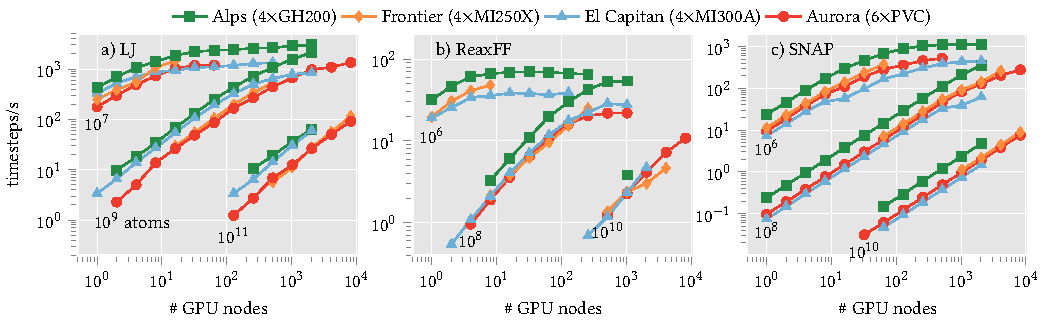
\includegraphics{generated-figures/paper-figure6.pdf}
\fi
\caption{Strong scaling results for LAMMPS on different exascale architectures. The total number of atoms is given by the label below each group of results. In cases of minor atom count discrepancies, the speed was rescaled assuming linear scaling. We see that SNAP, with its faster saturation (figure~\ref{fig:perfsat}) and higher computational expense delivers the best scaling, while ReaxFF with its lack of saturation plateau struggles to reach even 100 timesteps/s. Overall, we observe excellent strong scaling, even out to 8192 nodes on Frontier and El Capitan.}\label{fig:strongscaling}
\end{figure*}

\end{document}

